\documentclass[aspectratio=169]{beamer}

\usetheme{metropolis}

% Color scheme: Professional blues/teals
\definecolor{TechBlue}{HTML}{005587}
\definecolor{Teal}{HTML}{007C92}
\definecolor{LightTeal}{HTML}{E0F2F1}
\definecolor{AccentOrange}{HTML}{F57C00}
\definecolor{WarnRed}{HTML}{D32F2F}
\definecolor{GoodGreen}{HTML}{2E7D32}

\setbeamercolor{palette primary}{bg=TechBlue, fg=white}
\setbeamercolor{title separator}{fg=Teal}
\setbeamercolor{progress bar}{fg=Teal, bg=gray!20}
\setbeamercolor{alerted text}{fg=AccentOrange}
\setbeamercolor{block title alerted}{bg=AccentOrange!15, fg=AccentOrange!80!black}
\setbeamercolor{block body alerted}{bg=AccentOrange!5}

\usepackage{tikz}
\usetikzlibrary{shapes.geometric, arrows.meta, positioning, calc, fit, backgrounds}
\usepackage{booktabs}
\usepackage{graphicx}
\usepackage{amsmath}
\usepackage{fontawesome5}

\title{Ising-Edge}
\subtitle{Joint Compute Placement, Precision \& Low-Rank Compression\\via Quadratic Binary Optimisation for Snapdragon Edge AI}
\author{Jenish Patel}
\institute{Snapdragon AI Challenge 2026 \\ \small Track: On-Device Generative AI Acceleration \& Optimization}
\date{September 30, 2026}

\begin{document}

% ============================================================
% SLIDE 1: Title
% ============================================================
\maketitle

% ============================================================
% SLIDE 2: The Problem
% ============================================================
\begin{frame}{The Problem: No Single Engine Wins}
\begin{columns}[T]
\column{0.55\textwidth}
\textbf{Snapdragon SoCs} have 3 compute engines:
\begin{itemize}
    \item \textbf{Hexagon NPU} \textrightarrow{} Up to \alert{5$\times$ faster prefill}
    \item \textbf{CPU / GPU} \textrightarrow{} Up to \alert{2.5$\times$ faster decode}
\end{itemize}

\vspace{0.8em}
\textbf{Current approaches fail because:}
\begin{itemize}
    \item Placement, quantization, and compression are treated as \emph{disconnected} problems
    \item Compression damage is \emph{non-linear} and \emph{coupled} across layers
\end{itemize}

\column{0.42\textwidth}
\small
\begin{tabular}{@{}lcc@{}}
\toprule
\textbf{Engine} & \textbf{Prefill} & \textbf{Decode} \\
\midrule
NPU & \textcolor{GoodGreen}{\textbf{2,643}} & 45.9 \\
GPU & 665 & 42.8 \\
CPU & 353 & \textcolor{GoodGreen}{\textbf{47.9}} \\
\bottomrule
\end{tabular}
\vspace{0.3em}

\centering\scriptsize Galaxy S26, Qwen3-1.7B Q4\_0\\
512 context, tok/s\\[0.3em]
\scriptsize\textit{Source: Qualcomm perf.yaml}
\end{columns}
\end{frame}

% ============================================================
% SLIDE 3: Why It Matters
% ============================================================
\begin{frame}{The Compression Damage Trap}
\begin{columns}[T]
\column{0.58\textwidth}
\textbf{Single-layer planning is mathematically invalid.}

\vspace{0.5em}
Compressing 24 MLP blocks (layers 2--25):

\vspace{0.5em}
\begin{tabular}{@{}lr@{}}
\toprule
\textbf{Prediction Method} & $\Delta$\textbf{PPL} \\
\midrule
Linear sum of single layers & +57.8\% \\
Log-additive model & +76.8\% \\
\textbf{Actual measured} & \textcolor{WarnRed}{\textbf{+275.6\%}} \\
\bottomrule
\end{tabular}

\vspace{0.8em}
\textbf{4.8$\times$ underestimation} when ignoring cross-layer interactions.

\column{0.38\textwidth}
\centering
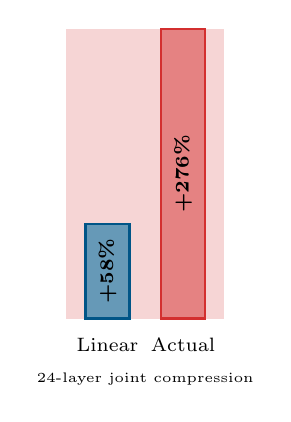
\begin{tikzpicture}[scale=0.8]
\fill[LightTeal] (0,0) rectangle (2.5,1.5);
\fill[WarnRed!20] (0,0) rectangle (2.5,4.6);
\draw[thick,TechBlue,fill=TechBlue!60] (0.3,0) rectangle (1.0,1.5);
\draw[thick,WarnRed,fill=WarnRed!60] (1.5,0) rectangle (2.2,4.6);
\node[font=\scriptsize\bfseries,rotate=90] at (0.65,0.75) {+58\%};
\node[font=\scriptsize\bfseries,rotate=90] at (1.85,2.3) {+276\%};
\node[font=\scriptsize,anchor=north] at (0.65,-0.15) {Linear};
\node[font=\scriptsize,anchor=north] at (1.85,-0.15) {Actual};
\node[font=\tiny,anchor=north] at (1.25,-0.7) {24-layer joint compression};
\end{tikzpicture}
\end{columns}
\end{frame}

% ============================================================
% SLIDE 4: Our Solution
% ============================================================
\begin{frame}{Ising-Edge: Unified QUBO Optimization}
\textbf{Jointly optimizes} across every transformer block:

\vspace{0.3em}
\begin{columns}[T]
\column{0.45\textwidth}
\begin{enumerate}
    \item \textbf{Compute placement} \textrightarrow{} CPU, GPU, NPU
    \item \textbf{Weight precision} \textrightarrow{} Q4\_0, Q8\_0
    \item \textbf{Compression level} \textrightarrow{} SVD \& MPO rank
\end{enumerate}

\vspace{0.8em}
All mapped into a single Ising Hamiltonian:
\[ \min_{x}\; \mathcal{H}(x) = c^T\!x + x^T\!Qx \]

\column{0.50\textwidth}
\begin{itemize}
    \item $c_i$: Isolated latency + accuracy penalty
    \item $Q_{ij}$: Hardware switching costs + \textbf{cross-layer perplexity coupling}
    \item Constraints: one-hot per layer, memory budget
\end{itemize}

\vspace{0.5em}
\alert{Output:} Native \texttt{llama.cpp} flags\\
\texttt{-dev HTP0,GPUOpenCL,none}\\
\texttt{-ot "blk.[0-12].*=HTP0"}\\
\texttt{-ctk q8\_0 -ctv q4\_0}
\end{columns}
\end{frame}

% ============================================================
% SLIDE 5: Architecture
% ============================================================
\begin{frame}{System Architecture}
\begin{center}
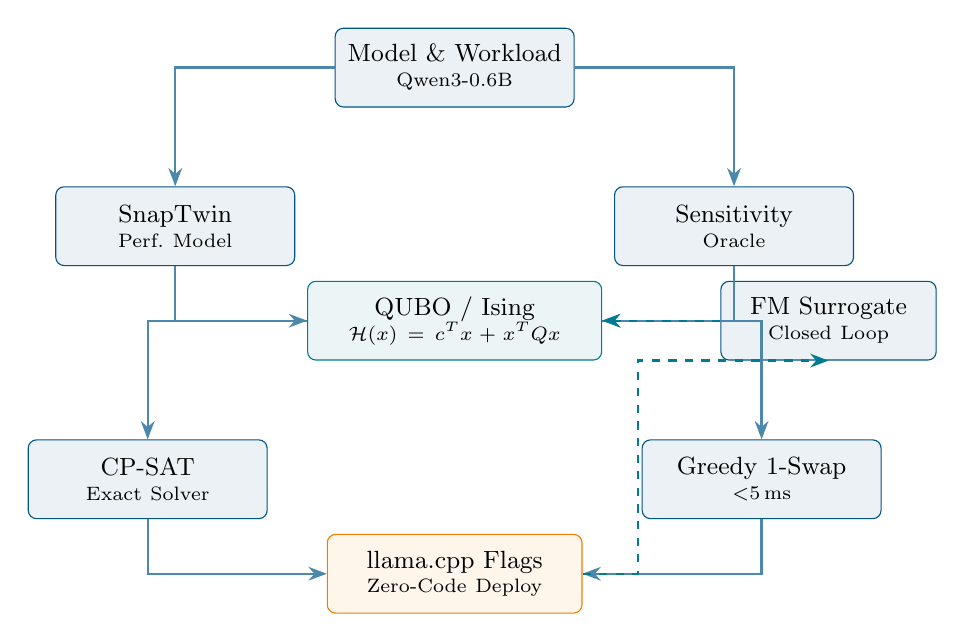
\begin{tikzpicture}[
    node distance=0.8cm and 1.2cm,
    box/.style={rectangle, draw=TechBlue, rounded corners=3pt, fill=TechBlue!8,
                text centered, font=\small, minimum height=1cm, text width=2.8cm},
    bigbox/.style={rectangle, draw=Teal, rounded corners=3pt, fill=Teal!8,
                   text centered, font=\small, minimum height=1cm, text width=3.5cm},
    outbox/.style={rectangle, draw=AccentOrange, rounded corners=3pt, fill=AccentOrange!8,
                   text centered, font=\small, minimum height=1cm, text width=3cm},
    arr/.style={-{Stealth[scale=1]}, thick, TechBlue!70}
]

% Row 1
\node[box] (model) {Model \& Workload\\[-2pt]\scriptsize Qwen3-0.6B};

% Row 2
\node[box, below left=1cm and 0.5cm of model] (twin) {SnapTwin\\[-2pt]\scriptsize Perf.\ Model};
\node[box, below right=1cm and 0.5cm of model] (oracle) {Sensitivity\\[-2pt]\scriptsize Oracle};

% Row 3
\node[bigbox, below=2.2cm of model] (qubo) {QUBO / Ising\\[-2pt]\scriptsize $\mathcal{H}(x) = c^Tx + x^TQx$};

% Row 4
\node[box, below left=1cm and 0.5cm of qubo] (cpsat) {CP-SAT\\[-2pt]\scriptsize Exact Solver};
\node[box, below right=1cm and 0.5cm of qubo] (swap) {Greedy 1-Swap\\[-2pt]\scriptsize $<$5\,ms};

% Row 5
\node[outbox, below=2.2cm of qubo] (deploy) {llama.cpp Flags\\[-2pt]\scriptsize Zero-Code Deploy};

% FM surrogate loop
\node[box, right=1.5cm of qubo, text width=2.5cm] (fm) {FM Surrogate\\[-2pt]\scriptsize Closed Loop};

% Arrows
\draw[arr] (model) -| (twin);
\draw[arr] (model) -| (oracle);
\draw[arr] (twin) |- (qubo);
\draw[arr] (oracle) |- (qubo);
\draw[arr] (qubo) -| (cpsat);
\draw[arr] (qubo) -| (swap);
\draw[arr] (cpsat) |- (deploy);
\draw[arr] (swap) |- (deploy);
\draw[arr, dashed, Teal] (fm) -- (qubo);
\draw[arr, dashed, Teal] (deploy.east) -- ++(0.7,0) |- (fm.south);

\end{tikzpicture}
\end{center}
\end{frame}

% ============================================================
% SLIDE 6: Result 1 — Matched Bytes
% ============================================================
\begin{frame}{Result: Combinatorial Superiority at Matched Bytes}
\begin{columns}[T]
\column{0.55\textwidth}
Under \textbf{strictly identical byte budgets} ($K\!=\!18$ MLPs at keep~0.8):

\vspace{0.5em}
\begin{tabular}{@{}llr@{}}
\toprule
\textbf{Budget} & \textbf{Plan} & $\Delta$\textbf{PPL} \\
\midrule
$K\!=\!6$ & Pairwise & \textcolor{GoodGreen}{\textbf{+6.76\%}} \\
$K\!=\!6$ & Random & +17.37\% \\
\midrule
$K\!=\!12$ & Pairwise & \textcolor{GoodGreen}{\textbf{+27.05\%}} \\
$K\!=\!12$ & Random & +36.83\% \\
\midrule
$K\!=\!18$ & Pairwise & \textcolor{GoodGreen}{\textbf{+66.90\%}} \\
$K\!=\!18$ & Random & +158.51\% \\
\bottomrule
\end{tabular}

\column{0.42\textwidth}
\centering
\vspace{1em}
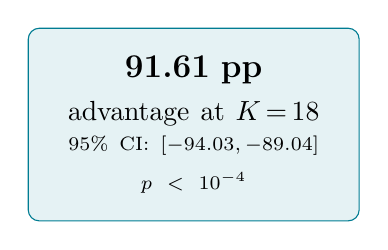
\begin{tikzpicture}
\node[draw=Teal, fill=Teal!10, rounded corners, inner sep=10pt, text width=3.5cm, align=center, font=\large] {
\textbf{91.61 pp}\\[0.3em]
\normalsize advantage at $K\!=\!18$\\[0.3em]
\scriptsize 95\% CI: $[-94.03, -89.04]$\\
\scriptsize $p < 10^{-4}$
};
\end{tikzpicture}
\end{columns}

\vspace{0.5em}
\small Paired bootstrap, 4,000 resamples. Full 584-chunk WikiText-2 evaluation.
\end{frame}

% ============================================================
% SLIDE 7: Result 2 — MPO vs SVD
% ============================================================
\begin{frame}{Result: Tensor Network Scaling (MPO vs.\ SVD)}
\begin{columns}[T]
\column{0.55\textwidth}
Across 24 layers (2--25) at \textbf{keep 0.9}, matched parameters:

\vspace{0.8em}
\begin{tabular}{@{}lrr@{}}
\toprule
\textbf{Method} & \textbf{PPL} & $\Delta$\textbf{PPL} \\
\midrule
Dense baseline & 21.884 & --- \\
\textbf{3-Core MPO} & \textcolor{GoodGreen}{\textbf{39.049}} & \textcolor{GoodGreen}{\textbf{+78.4\%}} \\
Activation SVD & 53.174 & +143.0\% \\
\bottomrule
\end{tabular}

\vspace{0.8em}
\textbf{$\sim$65 pp advantage} for MPO over SVD.

\column{0.42\textwidth}
\vspace{0.5em}
\textbf{Why MPO wins in deep composition:}

\vspace{0.5em}
\small
\begin{itemize}[nosep]
\item SVD errors \emph{align constructively} along residual stream
\item MPO distributes error \emph{isotropically} across tensor cores
\item Errors cancel \emph{destructively} over depth
\end{itemize}
\end{columns}
\end{frame}

% ============================================================
% SLIDE 8: Solver Performance
% ============================================================
\begin{frame}{Solver Performance: Discrete Dominates Continuous}
\vspace{0.3em}
\begin{table}[]
\centering
\begin{tabular}{@{}lrrrl@{}}
\toprule
\textbf{Solver} & \textbf{Optimality Gap} & \textbf{Runtime} & \textbf{Constraints} \\
\midrule
CP-SAT (Exact) & 0.000\% & 0.20--0.60\,s & Hard cuts \\
\rowcolor{GoodGreen!10}
\textbf{Greedy 1-Swap} & \textbf{0.000\%} & \textbf{$<$\,5\,ms} & \textbf{Feasible manifold} \\
Ballistic SB & 5.36--13.08\% & 0.31\,s & Penalty relaxation \\
Discrete SB & 19.11--44.79\% & 0.45\,s & Penalty relaxation \\
Simulated Annealing & 20.46--36.21\% & 2.10\,s & Penalty relaxation \\
\bottomrule
\end{tabular}
\end{table}

\vspace{0.5em}
\textbf{Key insight:} Hard equality constraints ($\sum x_i = K$) require penalty barriers $\lambda(\sum x_i - K)^2$ in continuous solvers, warping phase space. Greedy 1-swap operates \emph{directly on the feasible manifold}, evaluating swaps in $O(1)$ amortized time.
\end{frame}

% ============================================================
% SLIDE 9: Closed-Loop Surrogate
% ============================================================
\begin{frame}{Active Closed-Loop Planning}
\textbf{Measure $\to$ Fit $\to$ Solve} iterative refinement loop:

\vspace{0.5em}
\begin{columns}[T]
\column{0.55\textwidth}
\begin{itemize}
    \item Rank-6 Factorization Machine surrogate
    \item Fitted to $\ln(\text{PPL}/\text{PPL}_{\text{dense}})$
    \item CP-SAT acquisition over $9.9 \times 10^9$ feasible plans
    \item Dual strategy: exploitation + exploration
\end{itemize}

\vspace{0.5em}
\textbf{Result at $K\!=\!18$:}
\begin{itemize}
    \item Closed-loop: \textcolor{GoodGreen}{\textbf{+62.99\%}}
    \item One-shot: +64.52\%
    \item Random: +115--150\%
\end{itemize}

\column{0.42\textwidth}
\centering
\vspace{0.5em}
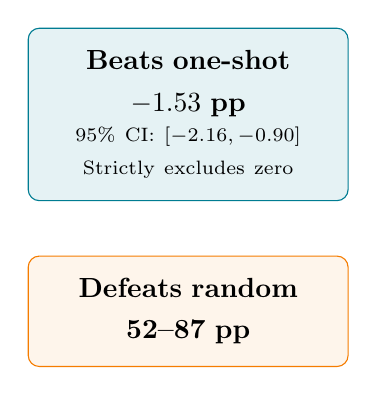
\begin{tikzpicture}
\node[draw=Teal, fill=Teal!10, rounded corners, inner sep=8pt, text width=3.5cm, align=center] {
\textbf{Beats one-shot}\\[0.3em]
\textbf{$-1.53$ pp}\\[0.3em]
\scriptsize 95\% CI: $[-2.16, -0.90]$\\
\scriptsize Strictly excludes zero
};

\vspace{0.8em}
\node[draw=AccentOrange, fill=AccentOrange!8, rounded corners, inner sep=8pt, text width=3.5cm, align=center] at (0,-2.5) {
\textbf{Defeats random}\\[0.3em]
\textbf{52--87 pp}
};
\end{tikzpicture}
\end{columns}
\end{frame}

% ============================================================
% SLIDE 10: Deployment
% ============================================================
\begin{frame}{Deployment: Zero-Code, Open-Source}
\begin{columns}[T]
\column{0.50\textwidth}
\textbf{100\% Open-Source Stack:}
\begin{itemize}
    \item \textbf{Qwen3-0.6B} (Apache-2.0)
    \item \textbf{llama.cpp} (MIT) with native\\Snapdragon backends
    \item WikiText-2, HotpotQA (public)
\end{itemize}

\vspace{0.5em}
\textbf{Native Flag Generation:}\\
Plans emit standard CLI parameters---no driver modifications required.

\column{0.45\textwidth}
\textbf{Quality Assurance:}
\begin{itemize}
    \item 56 unit tests, 100\% pass rate
    \item Automated numerical verification
    \item Cross-runtime validation
\end{itemize}

\vspace{0.5em}
\textbf{Target Platforms:}
\begin{itemize}
    \item Snapdragon X Elite / X2 Elite PCs
    \item Snapdragon 8 Gen 3 / 8 Elite phones
    \item Any \texttt{llama.cpp}-compatible device
\end{itemize}
\end{columns}
\end{frame}

% ============================================================
% SLIDE 11: Summary
% ============================================================
\begin{frame}{Key Takeaways}
\begin{center}
\Large\textbf{Ising-Edge: Unlocking Heterogeneous On-Device AI}
\end{center}

\vspace{0.5em}
\begin{columns}[T]
\column{0.30\textwidth}
\centering
\textbf{Unified\\Optimization}\\[0.5em]
\normalsize Jointly maps\\CPU/GPU/NPU,\\quantization \&\\low-rank compression\\into a single QUBO

\column{0.30\textwidth}
\centering
\textbf{Verified\\Accuracy Gains}\\[0.5em]
\normalsize \textbf{91.6 pp} advantage\\at matched bytes\\
\textbf{65 pp} MPO vs SVD\\
All with paired bootstrap CIs

\column{0.30\textwidth}
\centering
\textbf{Real-Time\\Edge Planning}\\[0.5em]
\normalsize \textbf{0\% gap} in $<$5\,ms\\
Native \texttt{llama.cpp}\\
Zero-code deploy\\
100\% open-source
\end{columns}

\vspace{1.5em}
\begin{center}
\large Thank you.
\end{center}
\end{frame}

\end{document}
